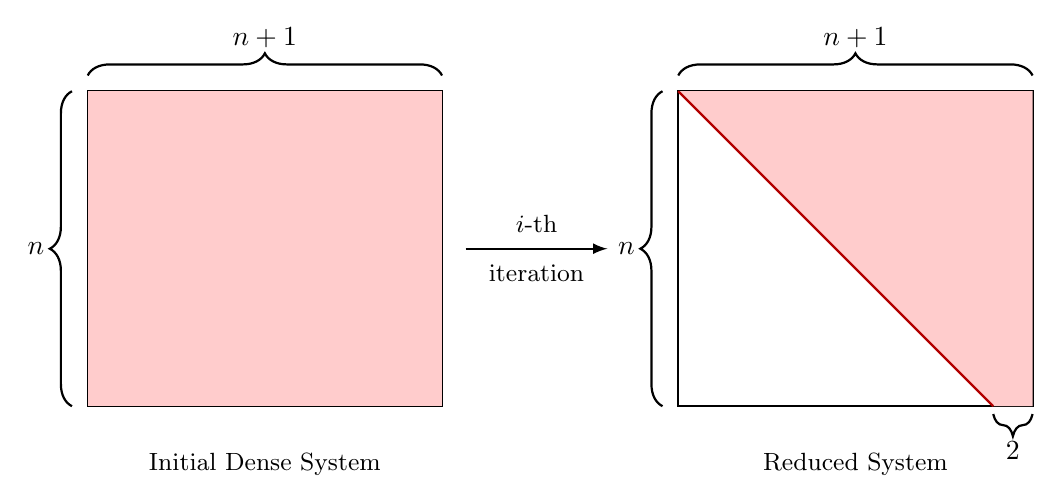
\begin{tikzpicture}[
    every node/.style={inner sep=0pt, outer sep=0pt},
    % Brace style
    curlybrace/.style={
        thick,
        decoration={brace, amplitude=8pt},
        decorate
    },
    % Matrix border style
    matrixbox/.style={
        draw=black,
        thick,
        fill=white
    }
]

% Global parameters (easy to scale)
\def\matH{4}       % Height of matrices (n)
\def\matW{4.5}     % Width of matrices (n+1)
\def\gap{3}        % Horizontal gap between matrices

% ================================
% 1. DENSE MATRIX (INITIAL SYSTEM)
% ================================
\begin{scope}[xshift=0cm]
    \draw[matrixbox] (0,0) rectangle (\matW,\matH);
    
    % Fully shaded
    \fill[fill=red!20] (0,0) rectangle (\matW,\matH);
    
    % Braces
    \draw[curlybrace] (-0.2,0) -- (-0.2,\matH) node[midway, left=10pt] {$n$};
    \draw[curlybrace] (0,\matH+0.2) -- (\matW,\matH+0.2) node[midway, above=10pt] {$n+1$};
    
    % Label below
    \node[anchor=north, font=\small] at (\matW/2, -0.6) {Initial Dense System};
\end{scope}

% ================================
% ARROW 1
% ================================
\draw[->, >=latex, thick] (\matW + 0.3, \matH/2) -- (\matW + \gap - 0.9, \matH/2)
    node[midway, above=6pt, font=\small, align=center] {$i$-th}
    node[midway, below=6pt, font=\small, align=center] {iteration};

% ================================
% 2. FINAL MATRIX (LINEAR RELATION)
% ================================
\begin{scope}[xshift=\matW cm + \gap cm]
    \draw[matrixbox] (0,0) rectangle (\matW,\matH);
    
    % Triangular shape
    \fill[fill=red!20] (0,\matH) -- (\matH,0) -- (\matW,0) -- (\matW,\matH) -- cycle;
    \draw[draw=red!70!black, thick] (0,\matH) -- (\matH,0);
    
    % Braces
    \draw[curlybrace] (-0.2,0) -- (-0.2,\matH) node[midway, left=10pt] {$n$};
    \draw[curlybrace] (0,\matH+0.2) -- (\matW,\matH+0.2) node[midway, above=10pt] {$n+1$};
    \draw[curlybrace] (\matW, -0.1) -- (\matH, -0.1) node[midway, below=10pt] {2};
    
    % Label below
    \node[anchor=north, font=\small] at (\matW/2, -0.6) {Reduced System};
\end{scope}

\end{tikzpicture}